\chapter{Конструкторская часть}

В данном разделе будут реализованы схемы алгоритмов нахождения расстояний Левенштейна и Дамерау\,--\,Левенштейна, приведено описание используемых типов данных, а также описана структура программного обеспечения.

\section{Требования к программному обеспечению}\label{section:requirements}
К программе предъявлен ряд требований:
\begin{itemize}[label=---]
	\item наличие интерфейса для выбора действий;
	\item возможность ввода строк;
	\item возможность обработки строк, включающих буквы как на латинице, так и на кириллице;
	\item возможность произвести замеры процессорного времени работы реализаций алгоритмов поиска расстояний Левенштейна и Дамерау\,--\,Левенштейна.
\end{itemize}

\section{Требования к вводу}\label{section:requirements}
\begin{enumerate}
    \item На вход подаются две строки;
    \item Буква нижнего и верхнего регистра считаются разными символами;
    \item Строки могут включать как символы латиницы, так и кириллицы.
\end{enumerate}

\section{Разработка алгоритмов}

На вход алгоритмов подаются строки $S_1$ и $S_2$.

На рисунке \ref{fig:Liter} представлена схема алгоритма поиска расстояния Левенштейна.
На рисунках \ref{fig:DLiter}--\ref{fig:DLrechash1} представлены схемы алгоритмов поиска Дамерау\,--\,Левенштейна.

\begin{figure}[h]
	\centering
	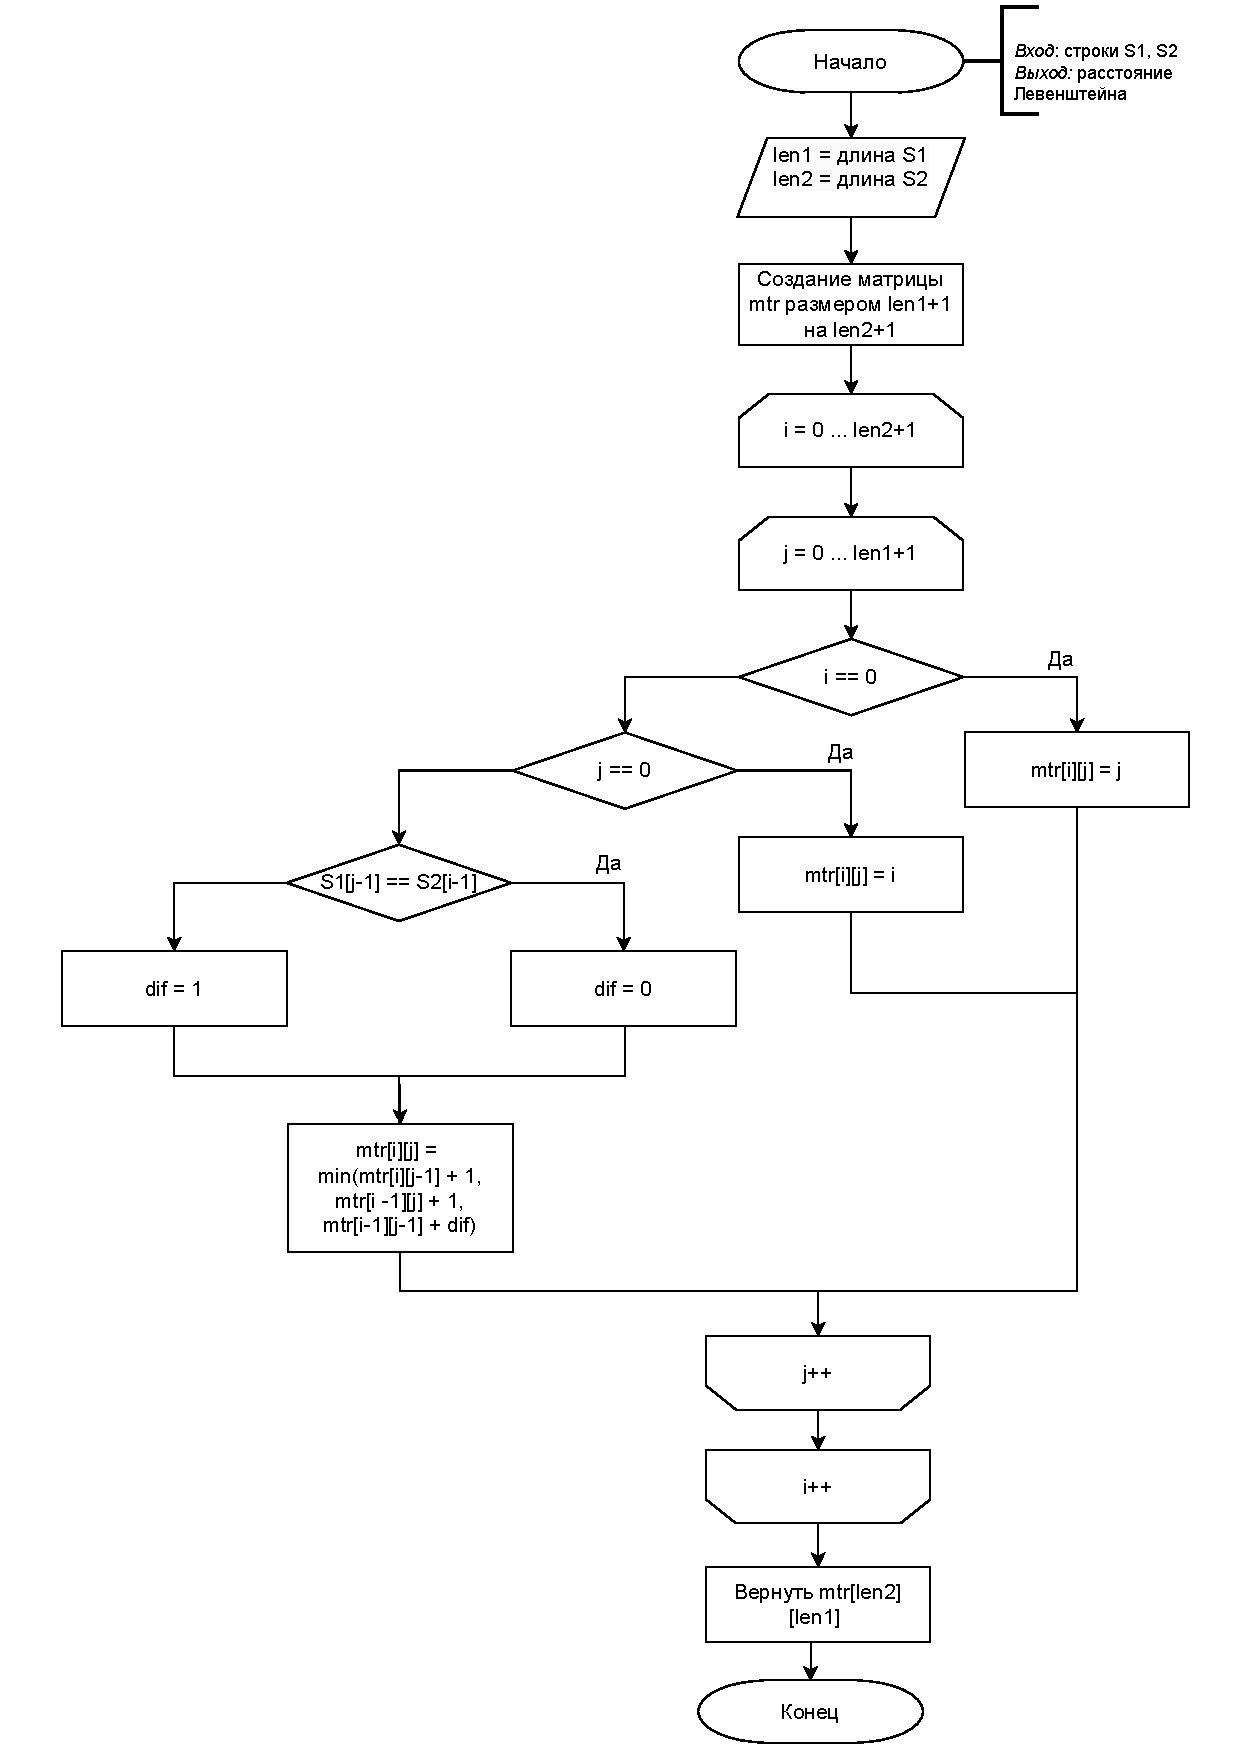
\includegraphics[height=0.7\textheight, page=1]{img/algoritms.pdf}
	\caption{Схема нерекурсивного алгоритма нахождения расстояния Левенштейна}
	\label{fig:Liter}
\end{figure}

\clearpage

\begin{figure}[h]
	\centering
	\includegraphics[height=0.9\textheight, page=2]{img/algoritms.pdf}
	\caption{Схема нерекурсивного алгоритма нахождения расстояния Дамерау\,--\,Левенштейна}
	\label{fig:DLiter}
\end{figure}

\clearpage

\begin{figure}[h]
	\centering
	\includegraphics[height=0.9\textheight, page=3]{img/algoritms.pdf}
	\caption{Схема рекурсивного алгоритма нахождения расстояния Дамерау\,--\,Левенштейна}
	\label{fig:DLrec}
\end{figure}

\clearpage

\begin{figure}[h]
	\centering
	\includegraphics[height=0.9\textheight, page=4]{img/algoritms.pdf}
	\caption{Схема рекурсивного алгоритма нахождения расстояния Дамерау\,--\,Левенштейна с кешированием}
	\label{fig:DLrechash1}
\end{figure}

\clearpage

\section{Описание используемых типов данных}

При реализации алгоритмов будут использованы следующие структуры данных:

\begin{itemize}
	\item \textit{строка}~--- массив типа $wchar{\_}t$ размером длины строки;
	\item \textit{длина строки}~--- целое число типа $int$;
	\item \textit{матрица}~--- двумерный массив значений типа $int$.
\end{itemize}

\section*{Вывод}

В данном разделе на основе теоретических данных были перечислены требования к ПО, а также были построены схемы требуемых алгоритмов на основе теоретических данных, полученных на этапе анализа.